\documentclass[12pt]{scrartcl}
\usepackage[a4paper,bindingoffset=0.2in,%
left=0.5in,right=0.5in,top=1in,bottom=1in,%
footskip=.25in]{geometry}
\usepackage[affil-it]{authblk}
\usepackage[utf8]{inputenc}
\usepackage{listings}
\usepackage{color}
\usepackage{xcolor}
\usepackage{pdfpages}
\usepackage{graphicx}
\graphicspath{{../images/}}
\usepackage{textcomp}
\usepackage{hyperref}
\usepackage{dirtree}
\usepackage{minted}
\usepackage{footnotebackref}

\definecolor{codegreen}{rgb}{0,0.6,0}
\definecolor{codegray}{rgb}{0.5,0.5,0.5}
\definecolor{codepurple}{rgb}{0.58,0,0.82}
\definecolor{backcolour}{rgb}{1.0,1.0,1.0}

\newcommand{\folder}[2]{}

\makeatletter
\newcommand\footnoteref[1]{\protected@xdef\@thefnmark{\ref{#1}}\@footnotemark}
\makeatother

\lstdefinestyle{mystyle}{
	backgroundcolor=\color{backcolour},   
	commentstyle=\color{codegreen},
	keywordstyle=\color{magenta},
	numberstyle=\tiny\color{codegray},
	stringstyle=\color{codepurple},
	basicstyle=\scriptsize,
	breakatwhitespace=false,         
	breaklines=true,                 
	captionpos=b,                    
	keepspaces=true
}


\lstset{style=mystyle}
\begin{document}
	\title{%
		Mercantile Ships
	}
	\author{Aly Shmahell\\%
		\href{aly.shmahell@gmail.com}{aly.shmahell@gmail.com}
	}
	\affil{%
		3rd Year Student\\
		Department of Computer Science, University of L'Aquila\\
		Databases - Lab Module\\
		Prof. Pierluigi Pierini
		}
	\date{Jan 9th 2018}
	
	\maketitle	
	\newpage
	\begin{center}
		\section*{\hfil \hfil  Abstract \hfil }
	\end{center}
		In this document I will showcase the 3 stages of design of the "Mercantile Ships" Database.\\
		In this effort, and under permission from the requirements file, I made some decisions regarding the techniques and tools used in the design process.\\
		In some extreme cases I had to settle for a less than optimal solution either for conformity purposes (the solution conforms best to the design stage) or for practicality, or for highlighting the optimal solution.\\
\newpage
\section*{\textbf{Design and Tool Choices}}
Having Ubuntu linux as my main operating system, I had a small set of tools to choose from, the obvious ones anyways.\\
For the Conceptual Schema, Dia was the most suggested on general forums, but it is highly outdated and full of bugs (as tested on my system), also it didn't offer any integrated features.\\

This is why I chose \textbf{MySQL Workbench}, it comes the most recommended from DB professionals, doesn't offer ER design capability, but better, it comes equipped with an EER designer, it offers backward engineering, forward engineering, SQL scripting, python scripting, SQL database connection, and with its SQL linter/debugger, the three stages of the DB design get improved live and professionally.\\

One note on MySQL Workbench, on its default settings, it only cares about relationships that translate into Foreign Keys, all other operations can be added as SQL routines(procedures)/triggers/scripts. Which makes sense, because this is how we actually translate from Conceptual Design to Logical Design.\\
But, the EER model in MySQL Workbench can be tweaked a little if someone wants to to add non-key-type relations. However, I chose to stick with the defaults.\\

Final note, MySQL Workbench provides both Conceptual EERD and Logical EERD: the first being offered with Crow's Foot Notation, the second with "Matching Columns to Columns" to simulate a graphical logical schema.\\

There are some other tools which I found (rather late), like draw.io, it's just a modeling tool, much like Dia, but it is more up to date and it has some nice features like adding your own shape (you have to script it in xml) so you can represent any special types of entities or relationships that are not present in the default palette.\\
Also, initially I only looked for tools concerning MySQL, but after doing a big portion of the project, I discovered pgModeler for PostgreSQL, which would have been better in terms of Conceptual Design because it represents non-key-type relations more out of the box and much better.\\

For testing the database I initially used phpMyAdmin, but due to its lack of proper support for delimiters in stored procedure I had to switch to \textbf{Adminer}.\\

As for the documentation, nothing beats \textbf{Latex} and \textbf{texstudio}!

\newpage
\section*{\normalsize{Conceputal Schema}}
In this schema I used Crow's Foot notation, mainly because it is the one adopted by the two CASE tools I used (MySQL WorkBench, draw.io).\\

With this notation, relationships cannot have attributes. Where necessary, relationships are promoted to entities in their own right. Where relationships are not promoted to entities, they represent external identifiers as foreign key or index attributes present in both entities on the left and right hand side.\\

This results in the following:
\begin{itemize}
	\item adaptation of external identifiers into foreign keys early on in the conceptual design stage.
	\item selection of primary identifiers can also be done in the conceptual design stage.
	\item many-to-many relationships are replaced with entities right in the conceptual design stage.
\end{itemize}
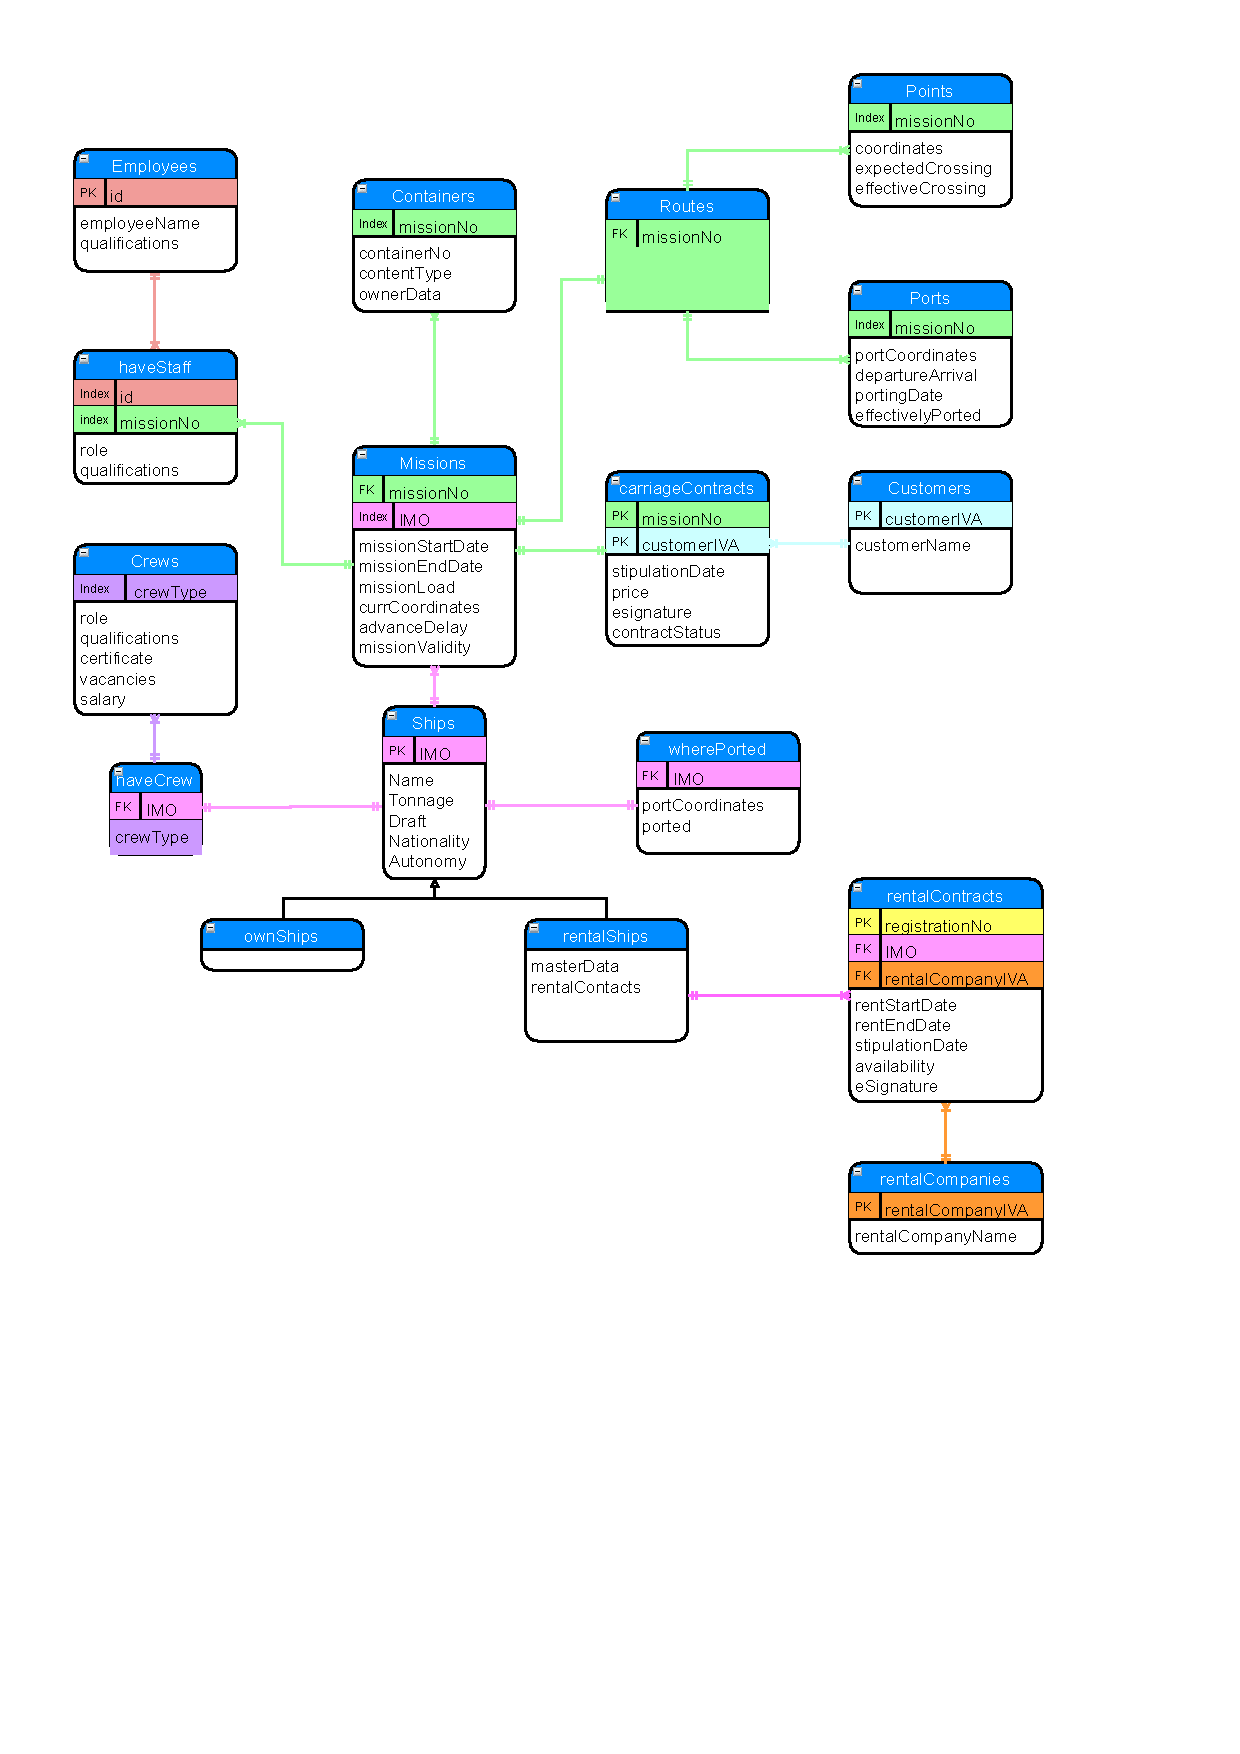
\includepdf[width=\textwidth, height=\textheight, pagecommand={\section*{\normalsize{Conceptual ERD with Crow's Foot (IE) Notation}} \thispagestyle{empty}}]{mercantileShips-Conceptual.pdf}
\newpage
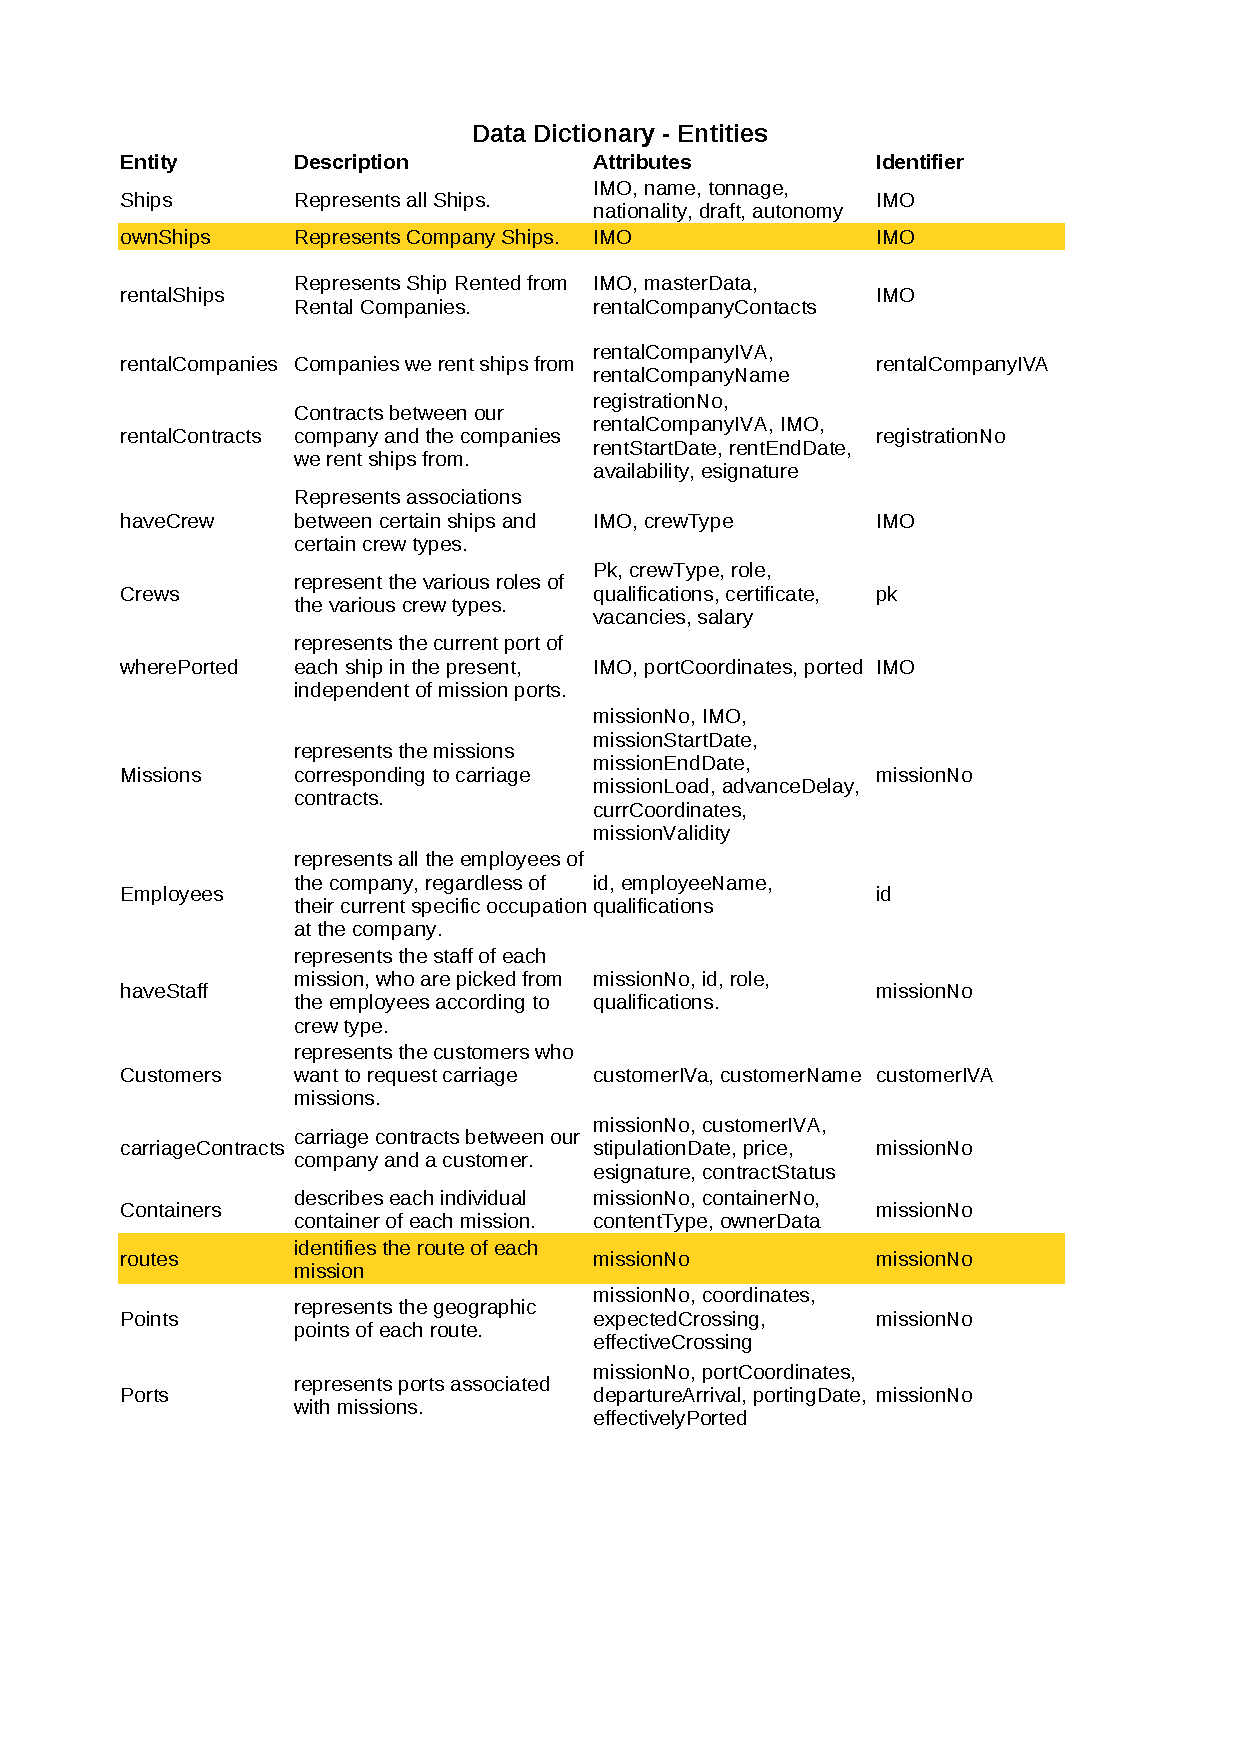
\includepdf[pagecommand={\thispagestyle{empty}}]{DataDictionary1.pdf}
\newpage
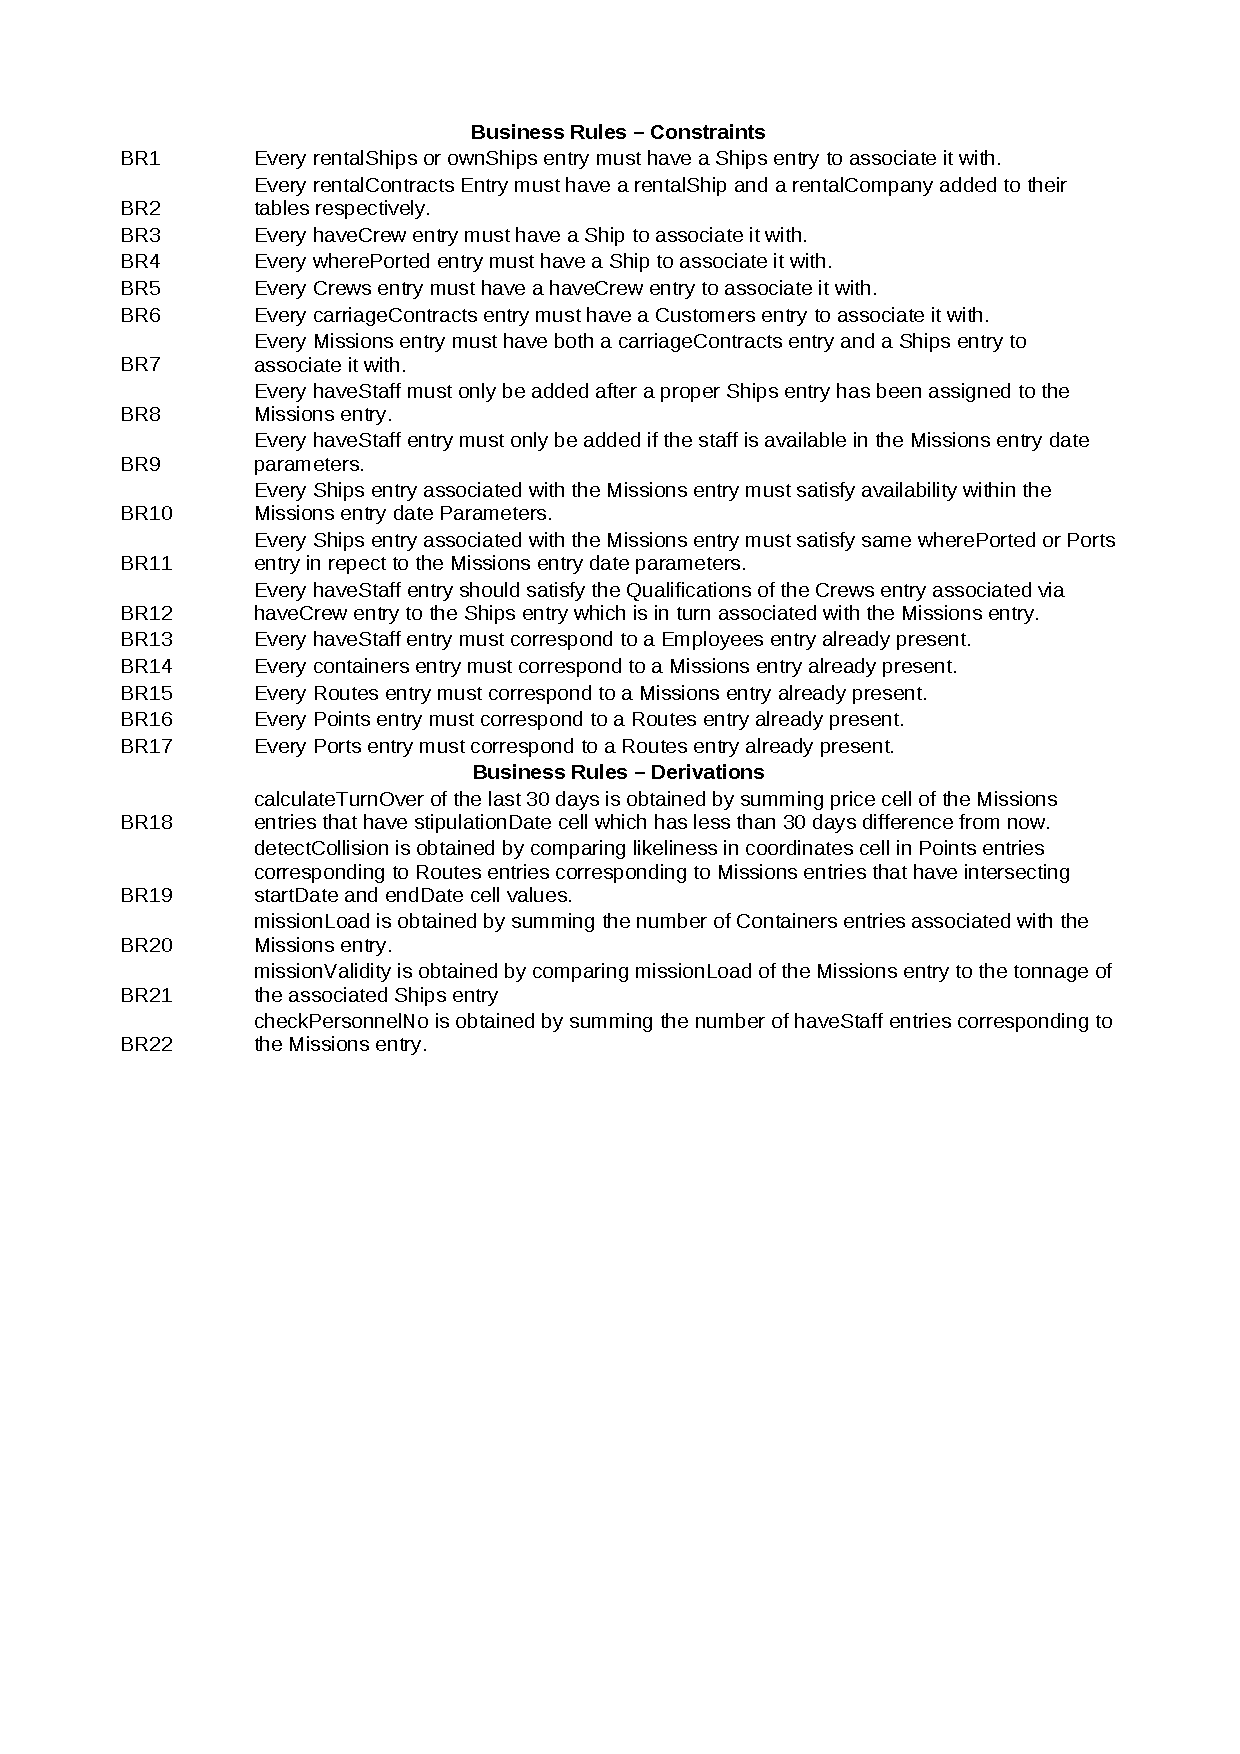
\includepdf[pagecommand={\thispagestyle{empty}}]{BusinessRules.pdf}
\newpage
\section*{\normalsize{From ER to Relational Model}}
During the Conceptual design stage I made sure to analyze and reduce redundancies as I was constructing the entities, I also made sure no entity crossed with another and therefor there was no need for collapse or merger of entities (except for the route entity which I alerted to its presence in the \hyperlink{page.13}{Notes on Efficiency} section).\\

The only thing left to do was removal of a generalization, which I chose to do it following the \textbf{"Substitution of the generalization with relationships"} method.\\

The resulting translated tables were as the following:
\begin{flushleft}
	Ships(\underline{IMO}, name, tonnage, draft, autonomy, nationality)\\
	ownShips(\underline{IMO})\\
	rentalShips(\underline{IMO}, masterData, rentalContacts)\\
	rentalCompanies(\underline{rentalCompanyIVA},rentalCompanyName)\\
	rentalContracts(\underline{registrationNo}, rentalCompanyIVA, IMO, rentStartDate, rentEndDate, availability, eSignature)\\
	wherePorted(\underline{IMO}, portCoordinates, ported)\\
	haveCrew(\underline{IMO}, crewType)\\
	Crews(\textit{crewType}, role, qualifications, certificate, vacancies, salary)\footnote{\label{italic1}attributes in italic represent indexes}\\
	Missions(\underline{missionNo}, IMO, missionStartDate, missionEndDate, missionLoad, currCoordinates, advanceDelay, missionValidity)\\
	Customers(\underline{customerIVA}, customerName)\\
	Employees(\underline{id}, employeeName, qualifications)\\
	carriageContracts(\underline{missionNo}, customerIVA, stipulationDate, price, eSignature, contractStatus)\\
	haveStaff (\textit{id}, \textit{missionNo}, role, qualifications)\footnoteref{italic1}\\
	Containers(\textit{missionNo}, containerNo, contentType, ownerData)\footnoteref{italic1}\\
	Routes(\underline{missionNo})\\
	Ports(\textit{missionNo}, portCoordinates, departureArrival, portingDate, effectivelyPorted)\footnoteref{italic1}\\
	Points(\textit{missionNo}, coordinates, expectedCrossing, effectiveCrossing)\footnoteref{italic1}\\
\end{flushleft}
\newpage
The resulting translated foreign key relations were as the following:
\begin{flushleft}
	\verb|fk_rentalContracts_rentalCompanies1|(rentalContracts.rentalCompanyIVA, rentalCompanies.rentalCompanyIVA)\\
	\verb|fk_rentalContracts_rentalShips1|(rentalContracts.IMO, rentalShips.IMO)\\
	\verb|fk_rentalShips_Ships1|(rentalShips.IMO,Ships.IMO)\\
	\verb|fk_ownShips_Ships1|(ownShips.IMO, Ships.IMO)\\
	\verb|fk_wherePorted_Ships1|(wherePorted.IMO, Ships.IMO)\\
	\verb|fk_haveCrew_Ships1|(haveCrew.IMO, Ships.IMO)\\
	\verb|fk_Crews_haveCrew1|(Crews.crewType, haveCrews.crewType)\\
	\verb|fk_Missions_Ships1|(Missions.IMO, Ships.IMO)\\
	\verb|fk_carriageContract_Customer1|(carriageContracts.customerIVA, Customers.customerIVA)\\
	\verb|fk_Missions_carriageContracts1|(Missions.MissionNo, carriageContracts.MissionNo)\\
	\verb|fk_haveStaff_Employees1|(haveStaff.id, Employees.id)\\
	\verb|fk_haveStaff_Missions1|(haveStaff.missionNo, Missions.missionNo)\\
	\verb|fk_Loads_Missions1|(Containers.missionNo, Missions.missionNo)\\
	\verb|fk_Routes_Missions1|(Routes.missionNo, Missions.missionNo)\\
	\verb|fk_Ports_Routes1|(Ports.missionNo, Routes.missionNo)\\
	\verb|fk_Points_Routes1|(Points.missionNo, Routes.missionNo)\\
\end{flushleft}
\newpage
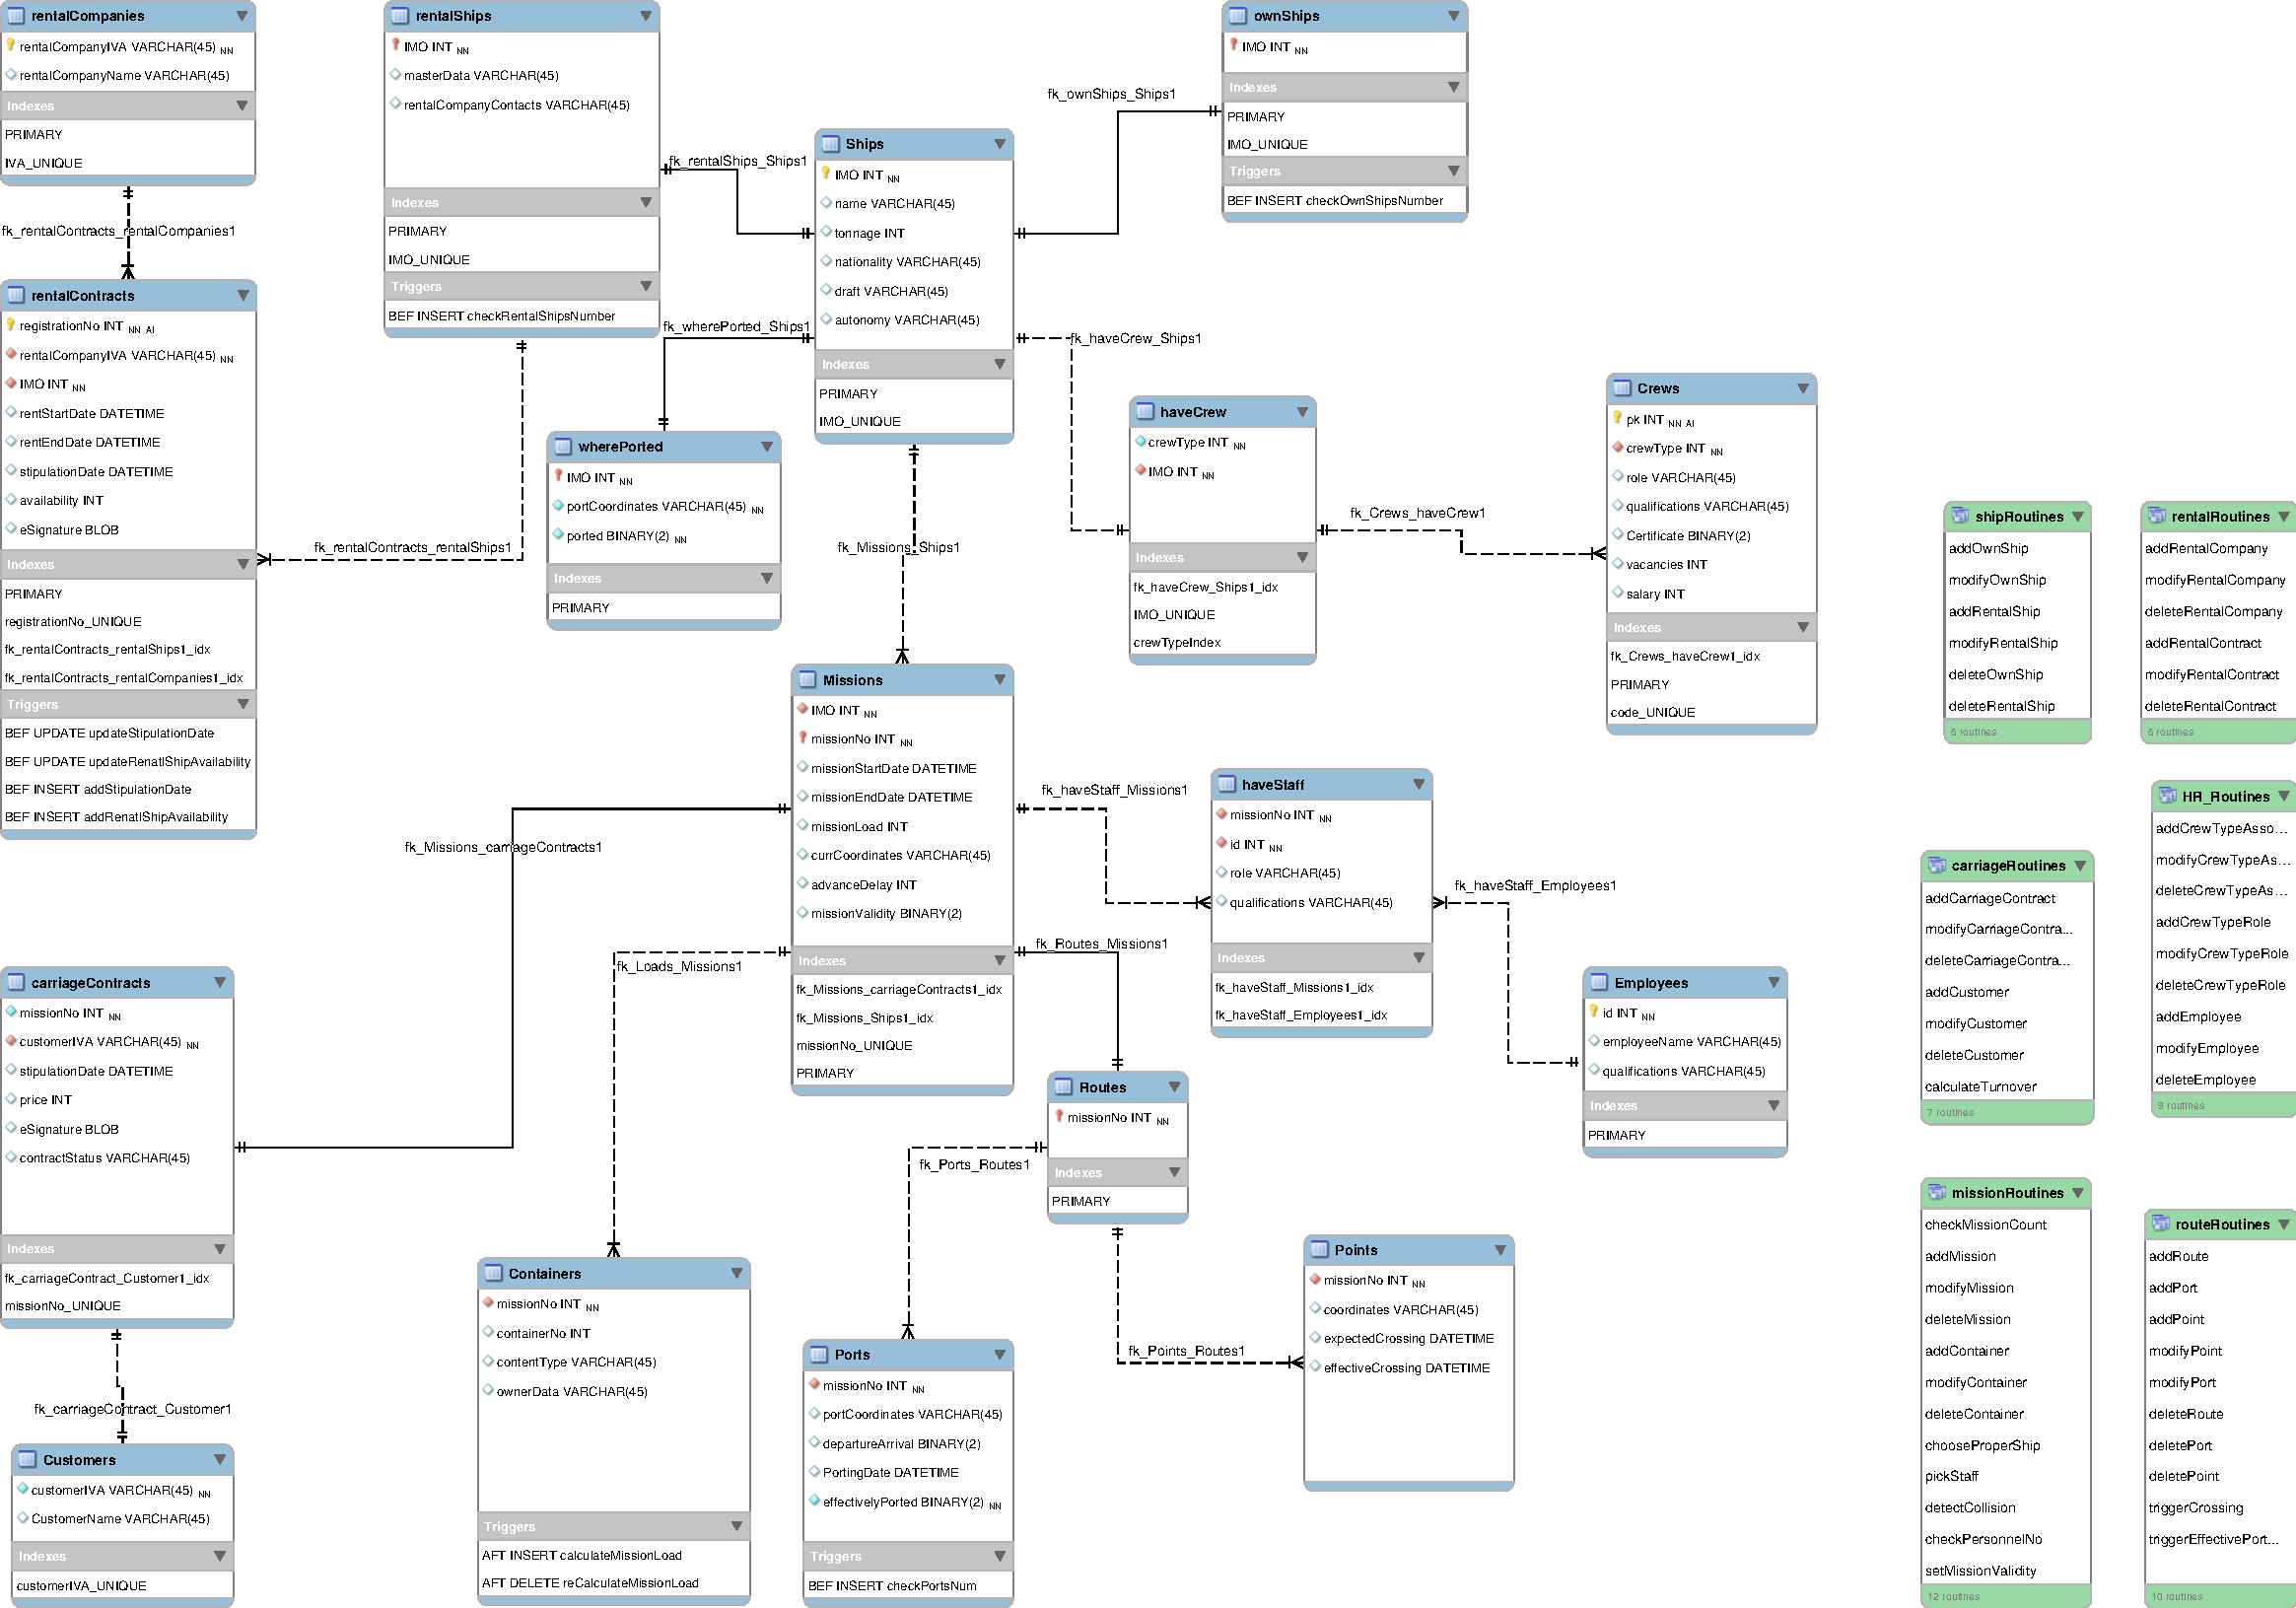
\includepdf[width=\textwidth, height=\textheight - 220pt, pagecommand={\section*{\normalsize{Relational EERD with Crow's Foot (IE) Notation}} \thispagestyle{empty}}]{MercantileShips-EER.pdf}
\newpage
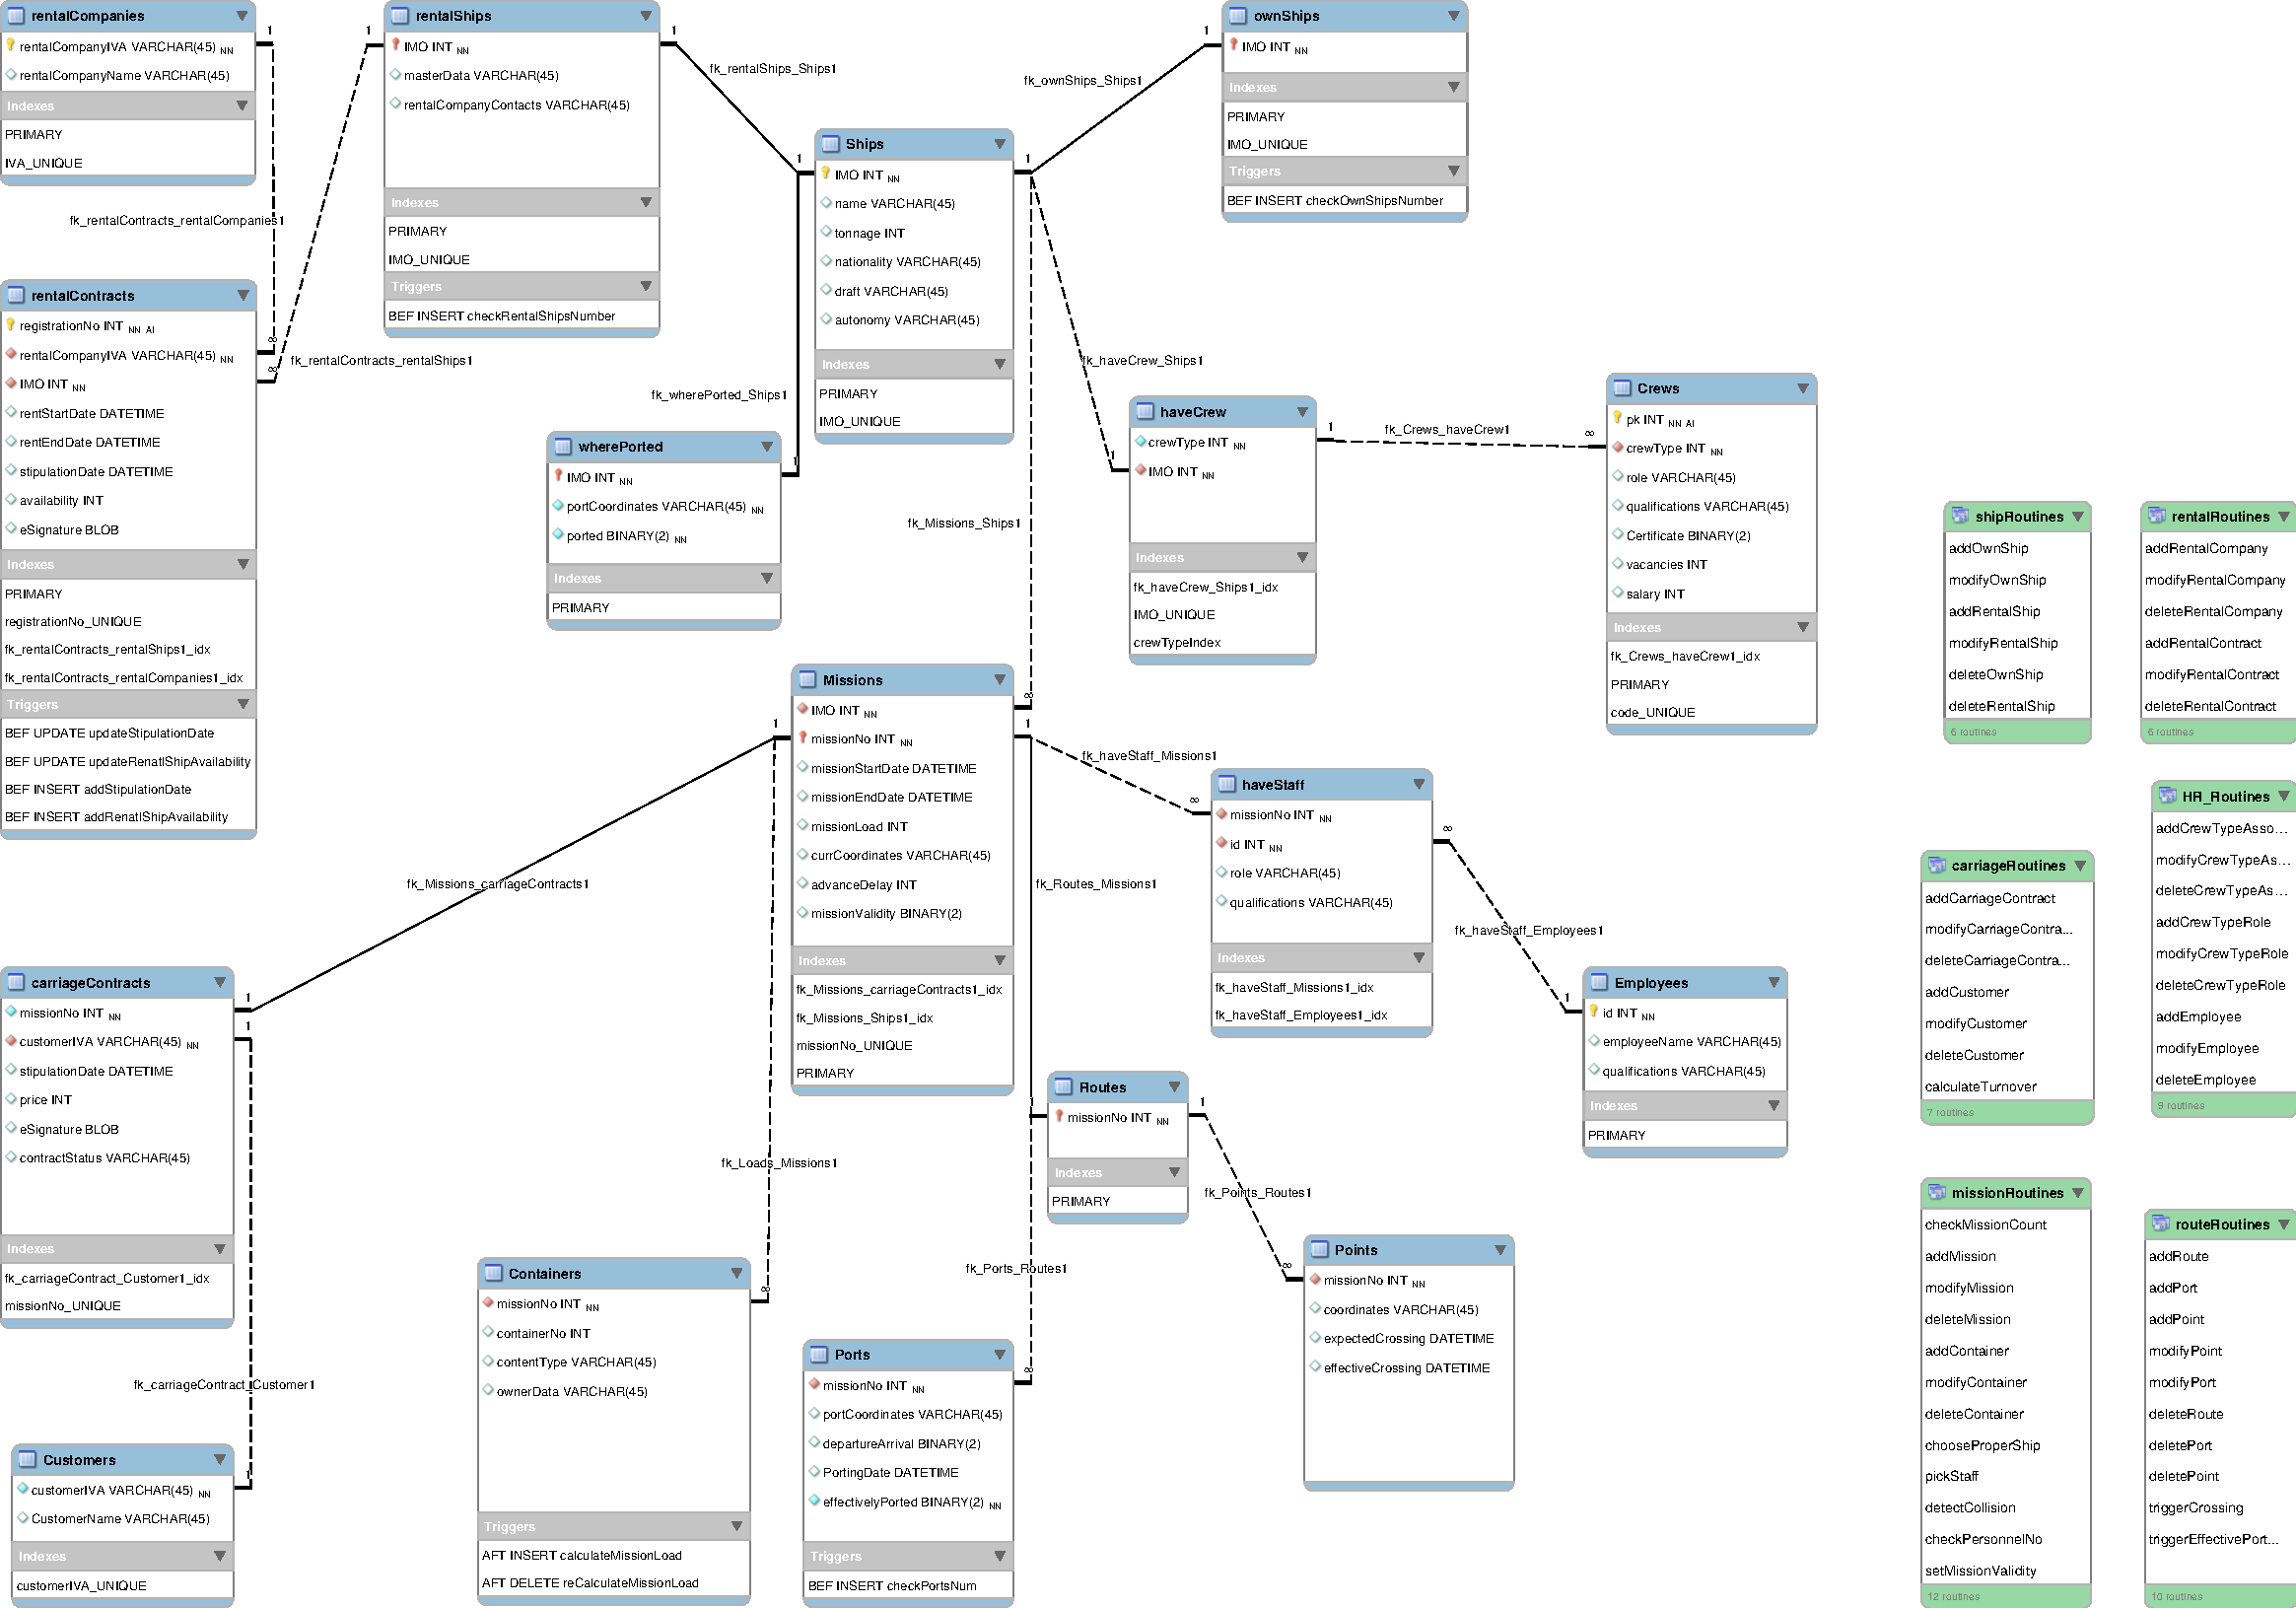
\includepdf[width=\textwidth, height=\textheight - 220pt, pagecommand={\section*{\normalsize{Logical EERD with Column Matching Notation }} \thispagestyle{empty}}]{MercantileShips-EER-Column.pdf}
\newpage
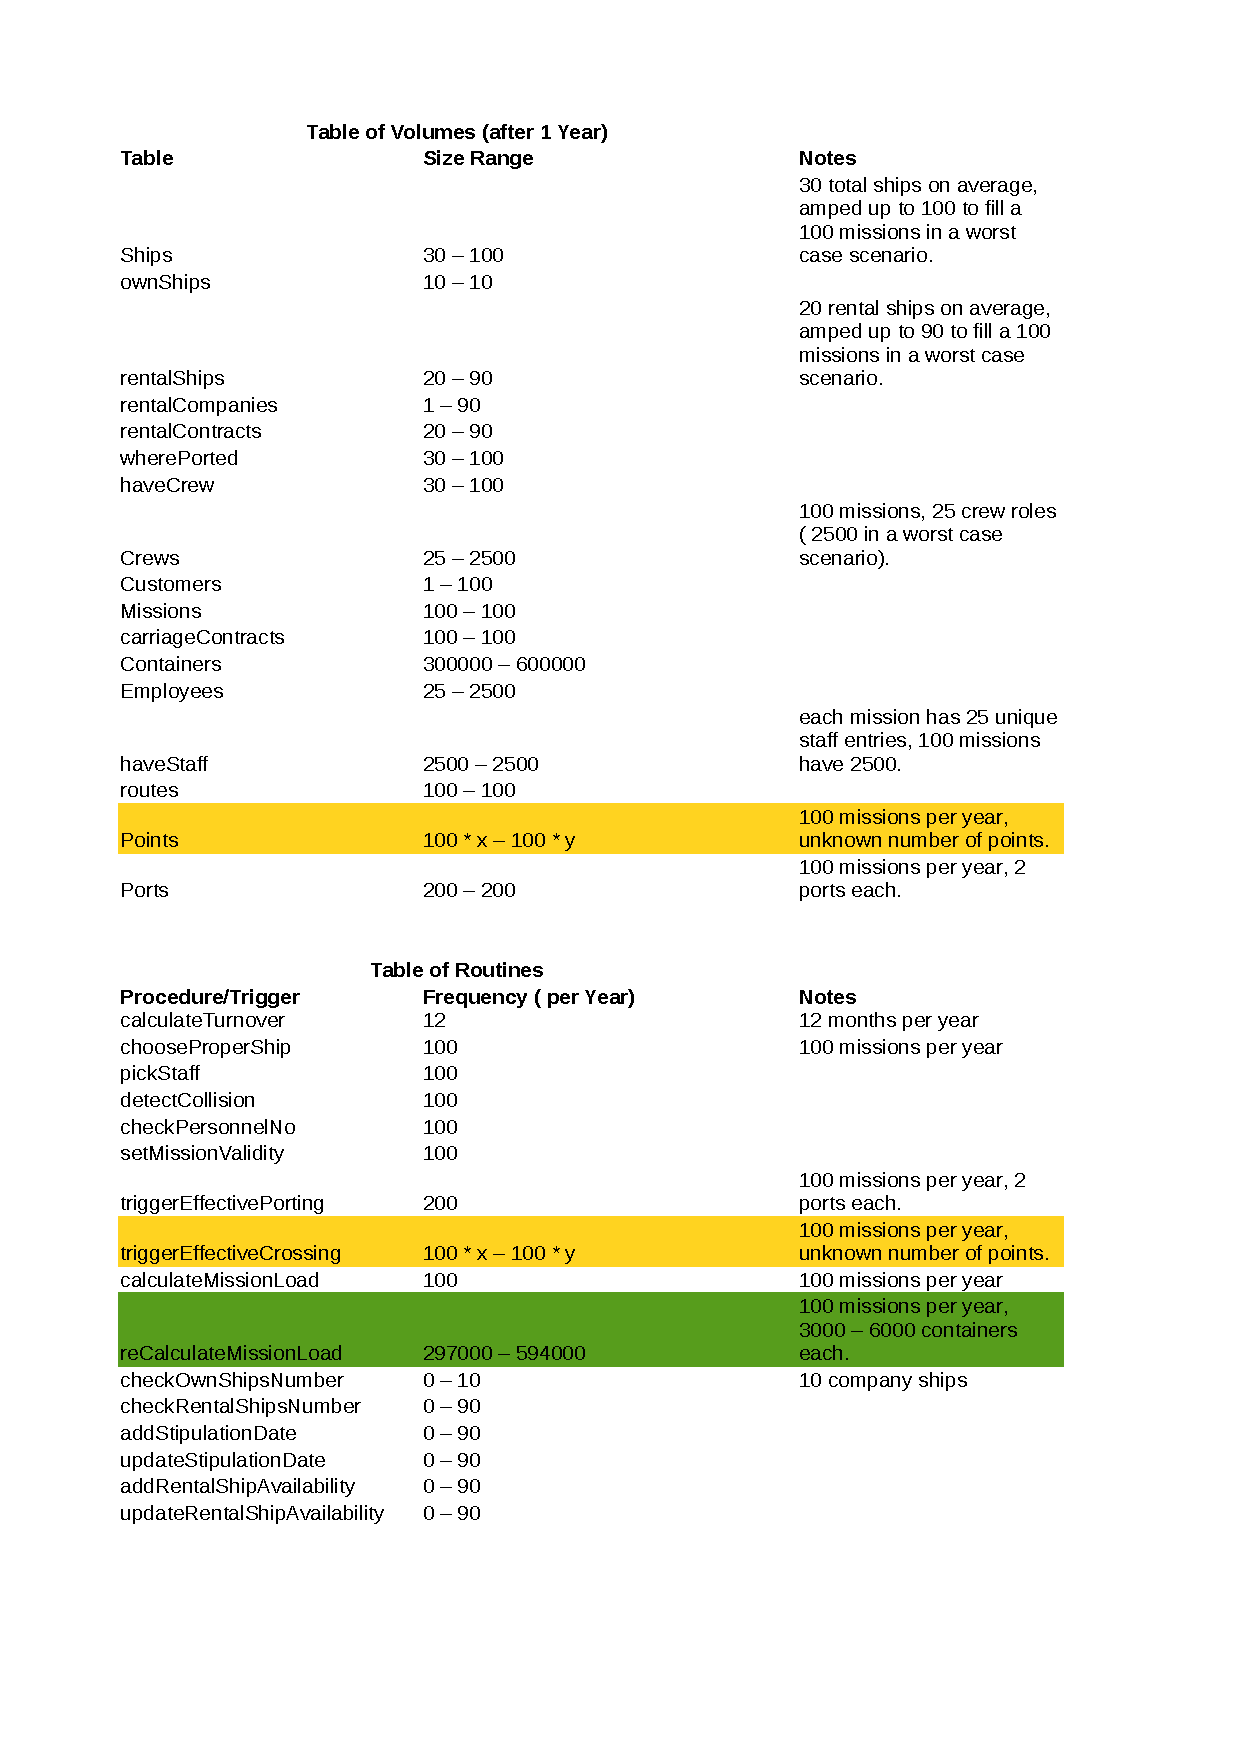
\includepdf[pagecommand={\thispagestyle{empty}}]{Volumes.pdf}
\newpage
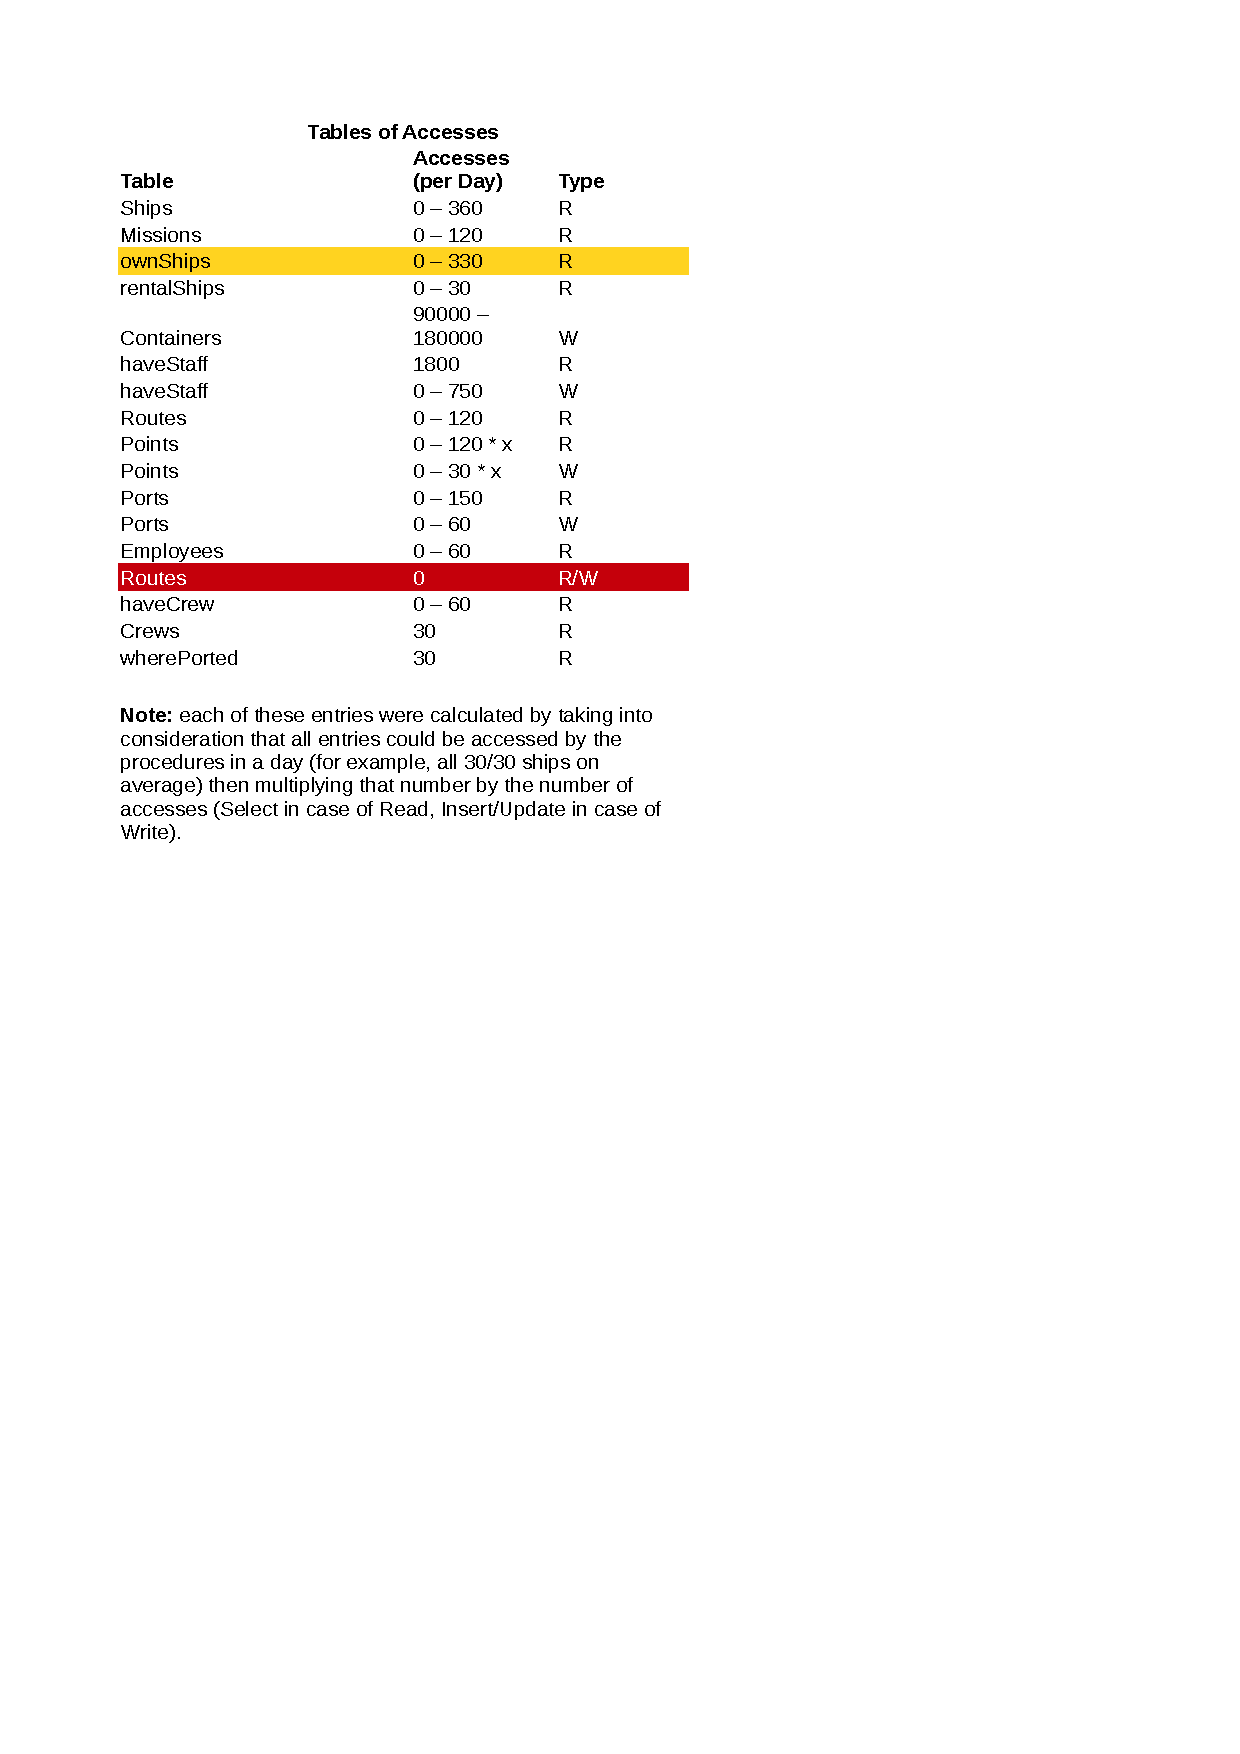
\includepdf[pagecommand={\thispagestyle{empty}}]{Accesses.pdf}
\subsection*{Notes on Efficiency}
As we can see in the table of accesses, the \textbf{Routes} table is accessed very rarely, and it imposes an un-necessary structural redundancy (only contains missionNo), therefor should be deleted and substituted with the \textbf{"missionNo"} attribute in the \textbf{Missions} table.\\

Also, the \textbf{ownShips} table is accessed as frequently as the \textbf{Ships} table, but poses another un-necessary structural redundancy, therefor should be deleted and substituted with a binary attribute \textbf{"isOwn"} in the \textbf{Ships} table.
\newpage
\section*{Physical Schema - MySQL Code (Tables, Constraints, Triggers, Procedures)}
\inputminted[breaklines=true, fontsize=\footnotesize]{mysql}{../../MySQL Code/AlyShmahell-mercantileShips.sql}
\newpage
\section*{Tool setup on Ubuntu 16.04 (Bash File)}
\inputminted[breaklines=true, fontsize=\footnotesize]{bash}{../../prerequisites.sh}
\newpage
\begin{flushleft}
	\section*{\textbf{Code Repository}}
\end{flushleft}
\begin{flushleft}
	A Github repository exists for this project under:\\
\end{flushleft}
	\begin{center}
		\url{https://github.com/AlyShmahell/Navibus-Mercatoriis}
	\end{center}
\begin{thebibliography}{}
\bibitem {MySQL 5.7 Reference Manual}
\textbf{MySQL 5.7 Reference Manual}: https://downloads.mysql.com/docs/refman-5.7-en.a4.pdf
\bibitem {MySQL Workbench 6.3 Reference Manual}
\textbf{MySQL Workbench 6.3 Reference Manual:} https://downloads.mysql.com/docs/workbench-en.a4.pdf
\end{thebibliography}
\end{document}
